%%%%%%%%%%%%%%%%%%%%%%%%%%%%%%%%%%%%
% template.tex
%
% Template for the KTHEEposter class.
%
% Original version: Mats Bengtsson, 28/5 2002
% Updated:
%   Mats Bengtsson April 2011 - July 2012
%   Manuel Olguín October 2018
%%%%%%%%%%%%%%%%%%%%%%%%%%%%%%%%%%%%

%\PassOptionsToPackage{showframe}{geometry}
\documentclass[portrait, a1]{KTHEEposter}
\usepackage{lipsum}
\usepackage{listings}
\usepackage{enumitem}
\usepackage[format=hang]{caption}
\usepackage{subcaption}
\captionsetup{font=normalsize,labelfont={bf,sf}}
\captionsetup[sub]{font={small}, textfont={normalfont}, labelfont={bf,sf}}
\usepackage{indentfirst}
\lstset{basicstyle=\ttfamily, frame=single}
\usepackage{pgfplots}
\pgfplotsset{compat=1.14}
\usepackage[export]{adjustbox}
\usepackage{tikz}
\usetikzlibrary{shapes,arrows.meta,positioning,automata}
\usepackage{sourcecodepro}
\usepackage{todonotes}
\usepackage{wrapfig}

\usepackage[style=ieee,
backend=bibtex,
sorting=none,
sortcites,
maxbibnames=1,
minbibnames=1,
maxcitenames=2, 
mincitenames=1]{biblatex}
\AtBeginBibliography{\footnotesize}
\addbibresource{bibliography.bib}


\kthlogo{kth_eng_cmyk}
\extralogo{img/cmu_csd_logo}
\kthcolor{KTHblue}

\begin{document}

\title{\Huge{\bfseries EdgeDroid 1.0}\\\normalfont\LARGE An Experimental Approach to Benchmarking Human-in-the-Loop Applications}

\author{\Large Manuel Olguín, Junjue Wang,\\Mahadev Satyanarayanan, James Gross}
\maketitle

\begin{pcolumns}[3]
    \begin{pcolumn}[2]
        \begin{pframe}[.75]
            \section{Abstract}
            Many emerging mobile applications, including augmented reality (AR) and wearable cognitive assistance, aim to provide seamless user interaction.
            However, the complexity of benchmarking these human-in-the-loop applications limits reproducibility and makes performance evaluation difficult. In this paper, we present EdgeDroid, a benchmarking suite designed to reproducibly evaluate these applications.

            Our core idea rests on recording traces of user interaction, which are then replayed at benchmarking time in a controlled fashion based on an underlying model of human behavior.
            This allows for an automated system that greatly simplifies benchmarking large scale scenarios and stress testing the application.
            Our results show the benefits of EdgeDroid as a tool for both system designers and application developers.
        \end{pframe}
        \begin{pframe}[1.25]
            \section{Basic Idea}
            \begin{itemize}
                \item Benchmarking human-in-the-loop applications is \textbf{hard} due to human users:
                      \begin{itemize}
                          \item They are unpredictable.
                          \item They make scaling difficult (you need more of them!).
                      \end{itemize}
                \item What if we could cut out the user?
            \end{itemize}
            \medskip
            \begin{center}
                \medskip
                \makeatletter
                \let\theoldfigure=\fnum@figure
                \renewcommand{\fnum@figure}{Step~\thefigure}
                \makeatother
                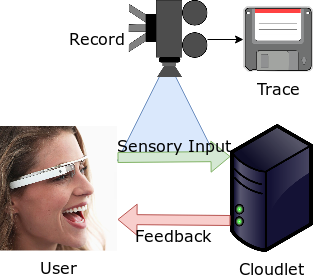
\includegraphics[width=.7\linewidth]{img/trace_idea_1}
                \captionof{figure}{Trace user input while operating the target application.}

                \medskip\medskip

                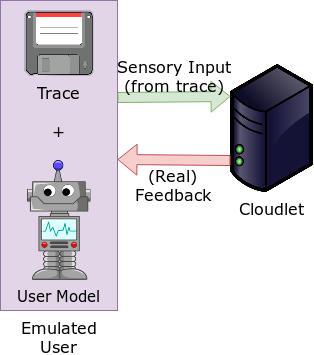
\includegraphics[width=.7\linewidth]{img/trace_idea_2}
                \captionof{figure}{Replace user with recorded trace plus a user model.}
                \makeatletter
                \renewcommand{\fnum@figure}{\theoldfigure}
                \makeatother
                \setcounter{figure}{0}
            \end{center}

        \end{pframe}
    \end{pcolumn}%
    \begin{pcolumn}[2]
        \begin{pframe}[.9]
            \section{Design \& Implementation}
            \begin{center}
                \medskip
                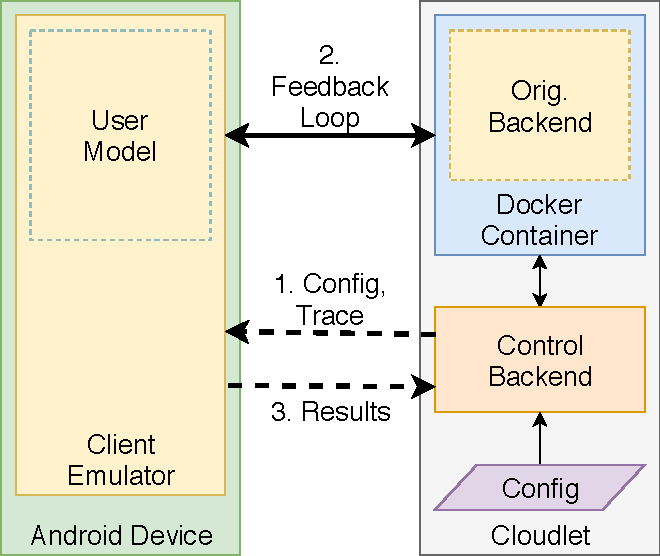
\includegraphics[width=.9\linewidth]{img/TraceReplay_GenArch}
                \captionof{figure}{Suite Architecture}
                \medskip
            \end{center}
            \begin{itemize}
                \item The \emph{control backend} controls the experiments and collects measurements from the application and the cloudlet itself.
                Implemented in Python~3.6.
                \item The \emph{client~emulators} play out a pre-recorded sensory input trace over the network in a controlled fashion, while collecting relevant metrics.
                Implemented in Java using the Android~SDK.%
            \end{itemize}
        \end{pframe}
        \begin{pframe}[1.1]
            \section{User Model}
            \begin{center}
                \medskip
                \adjustbox{scale=0.7}{
    \ttfamily\centering%\fbox{%
    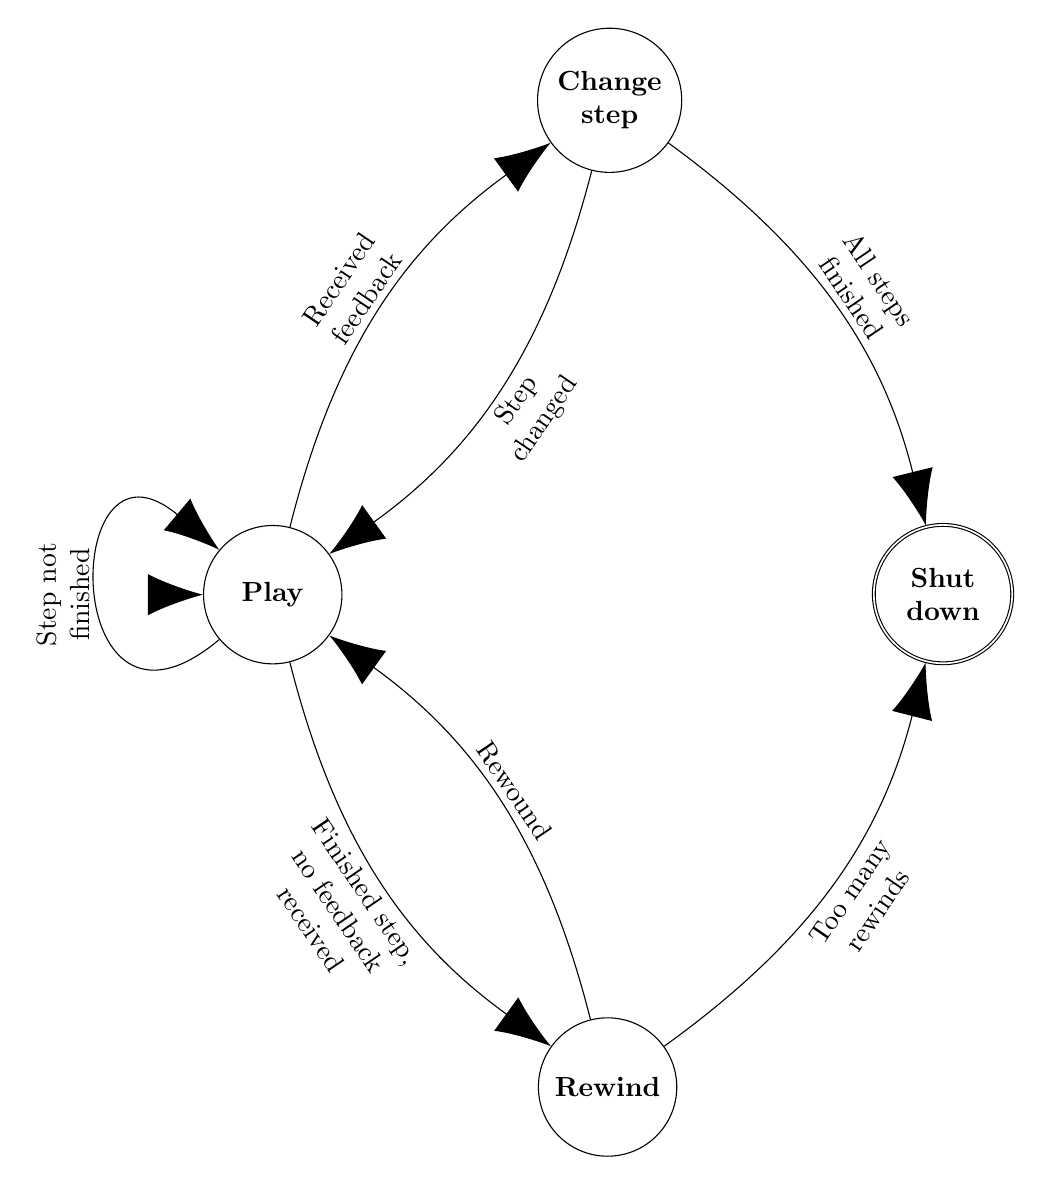
\begin{tikzpicture}[align=center,
        node distance=5cm and 3cm,
        every initial by arrow/.style={-{Latex[length=7mm]}}]
        % Place nodes              
        \node [initial, state, minimum size=5em, initial text=] (play) {\textbf{Play}};
        \node [state, above right=of play, minimum size=5em] (change) {\textbf{Change}\\\textbf{step}};
        \node [state, below right=of play, minimum size=5em] (rewind) {\textbf{Rewind}};
        \node [state, accepting, above right=of rewind, minimum size=5em] (shutdown) {\textbf{Shut}\\\textbf{down}};

        % Draw edges
        \path[draw, -{Latex[length=7mm]}, sloped, anchor=center]
        (play) edge [bend right=20] node[below] {Finished step,\\no feedback\\received} (rewind)
        edge [bend left=20] node[above] {Received\\feedback} (change)
        edge [in=140, out=220,looseness=6] node[above] {Step not\\finished} (play)

        (change) edge [bend left=20] node[below] {Step\\changed} (play)
        edge [bend left=20] node[above] {All steps\\finished} (shutdown)

        (rewind) edge [bend right=20] node[above] {Rewound} (play)
        edge [bend right=20] node[below] {Too many\\rewinds} (shutdown);

    \end{tikzpicture}
}%}
                \captionof{figure}{Model of human interaction.}
                \medskip
            \end{center}

            We implement a very simple user model in order to be able to react to feedback from the application and adapt our replay of the trace to the current system conditions.
            In EdgeDroid 1.0, our model is that of a user who does not suffer any of the shortcomings of real human users such as annoyance, fatigue, frustration, nausea.            
            In the future, we envision creating  many versions of EdgeDroid (i.e., EdgeDroid 2.0, EdgeDroid 3.0, etc.) that embody more human-like user models that more accurately emulate attributes such as those mentioned above. 
        \end{pframe}%    
    \end{pcolumn}%
    \begin{pcolumn}[2]
        \begin{pframe}[1.55]
            \section{Some Example Results}
            \begin{center}
                \medskip
                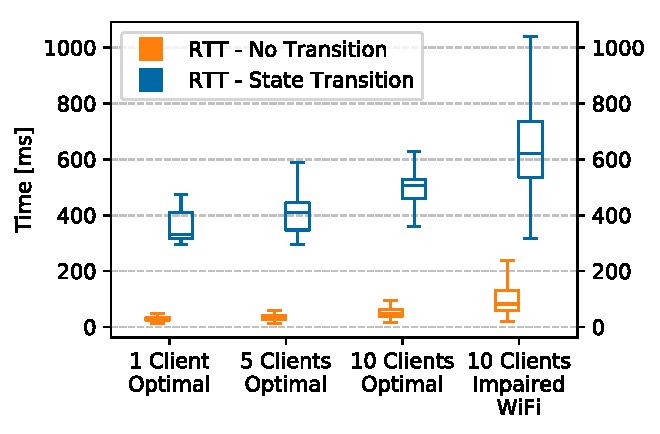
\includegraphics[width=\linewidth]{plots/comparison/rtt_fb_vs_nofb.pdf}
                \captionof{subfigure}{Comparison of total RTTs.}
                \medskip
                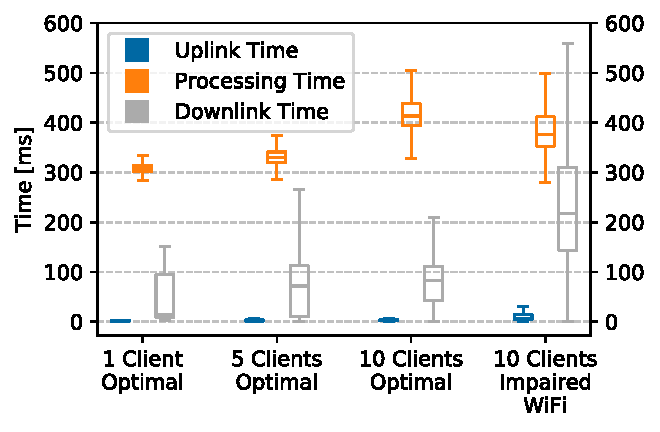
\includegraphics[width=\linewidth]{plots/comparison/box_feedback.pdf}
                \captionof{subfigure}{RTTs by major pipeline segments.}
                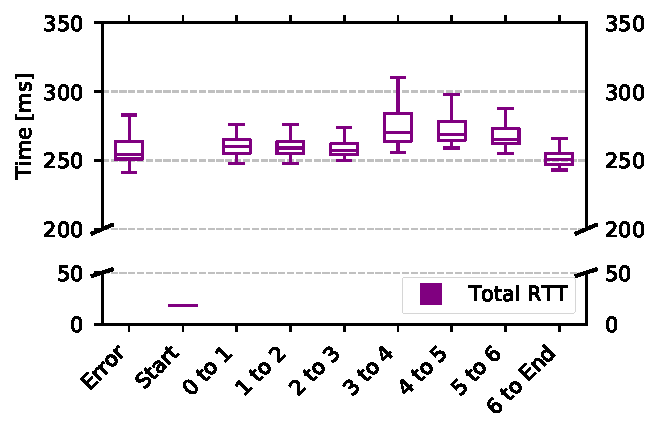
\includegraphics[width=\linewidth]{plots/comparison/box_taskstep.pdf}
                \captionof{subfigure}{RTTs by step transition.}
                \captionof{figure}{Example results for a benchmark of the LEGO application in~\cite{Chen:EarlyImplementation}.}
                \medskip
            \end{center}

            These results could be useful for:
            \begin{itemize}
                \item System designers wishing to identify bottlenecks in their hardware stack.
                \item Application developers who want to find potential for optimization.
            \end{itemize}
        \end{pframe}
        \begin{pframe**}[.45]
            \nocite{*}
            \footnotesize
            \printbibliography
        \end{pframe**}
    \end{pcolumn}
\end{pcolumns}

\end{document}

% \begin{pframe}[.17]
%     \medskip\itshape\footnotesize
%     We will eventually make the benchmark suite available as Free and Open Source Software.
%     The traces will also be made available under a Creative Commons License.
% \end{pframe}